

\documentclass[12pt,a4paper]{article}

\RequirePackage[hmargin=2.5cm,vmargin=2.5cm]{geometry}

\usepackage[T1]{fontenc}
\usepackage{lmodern}
\usepackage{amssymb,amsmath}
\usepackage{tcolorbox}
\usepackage{textcomp}
\usepackage{ifxetex,ifluatex}
\usepackage{fixltx2e} % provides \textsubscript
\usepackage{mathptmx}
\usepackage{caption}

\usepackage{lineno}


\usepackage{csvsimple}

\DeclareCaptionFont{xipt}{\fontsize{12}{14}\mdseries}
\usepackage[margin=10pt,font=xipt,labelfont=bf,justification=raggedleft]{caption}
\usepackage{wrapfig}

\usepackage{longtable}
\usepackage{booktabs}

%ns
\usepackage{colortbl}
\usepackage{pifont}
%

\usepackage{fontspec}
\usepackage{xcolor}

\usepackage{titlesec}
\defaultfontfeatures{Ligatures=TeX}
\setsansfont{Times New Roman}
\setmainfont{Times New Roman}

\pagenumbering{gobble}

\usepackage{array}
\newcolumntype{L}[1]{>{\raggedright\let\newline\\\arraybackslash\hspace{0pt}}m{#1}}
\newcolumntype{C}[1]{>{\centering\let\newline\\\arraybackslash\hspace{0pt}}m{#1}}
\newcolumntype{R}[1]{>{\raggedleft\let\newline\\\arraybackslash\hspace{0pt}}m{#1}}



% Set formats for each heading level
\titleformat*{\section}{\fontsize{12}{14}\bfseries\sffamily}
\titleformat*{\subsection}{\fontsize{12}{14}\bfseries\sffamily}
\titleformat*{\subsubsection}{\itshape\fontsize{12}{14}\sffamily}

% set title space
%\titlespacing{command}{left spacing}{before spacing}{after spacing}[right]
% spacing: how to read {12pt plus 4pt minus 2pt}
%           12pt is what we would like the spacing to be
%           plus 4pt means that TeX can stretch it by at most 4pt
%           minus 2pt means that TeX can shrink it by at most 2pt
%       This is one example of the concept of, 'glue', in TeX

\titlespacing\section{0pt}{10pt plus 4pt minus 2pt}{6pt plus 2pt minus 2pt}
\titlespacing\subsection{0pt}{10pt plus 4pt minus 2pt}{0pt plus 2pt minus 2pt}
\titlespacing\subsubsection{0pt}{10pt plus 4pt minus 2pt}{0pt plus 2pt minus 2pt}



% Reduce space in lists
\usepackage{enumitem}
\setlist{nosep} % or \setlist{noitemsep} to leave space around whole list




\usepackage{graphicx}
% We will generate all images so they have a width \maxwidth. This means
% that they will get their normal width if they fit onto the page, but
% are scaled down if they would overflow the margins.
\makeatletter
\def\maxwidth{\ifdim\Gin@nat@width>\linewidth\linewidth
\else\Gin@nat@width\fi}
\makeatother
\let\Oldincludegraphics\includegraphics
\renewcommand{\includegraphics}[1]{\Oldincludegraphics[width=\maxwidth]{#1}}

\usepackage{caption}
\captionsetup[figure]{labelfont={bf}, justification=raggedright, singlelinecheck=false, font={stretch=1.5}}
\usepackage[labelsep=none]{caption}

% fix floating figures
\usepackage{float}
\let\origfigure\figure
\let\endorigfigure\endfigure
\renewenvironment{figure}[1][2] {
    \expandafter\origfigure\expandafter[H]
} {
    \endorigfigure
}


\ifxetex
  \usepackage[setpagesize=false, % page size defined by xetex
              unicode=false, % unicode breaks when used with xetex
              xetex]{hyperref}
\else
  \usepackage[unicode=true]{hyperref}
\fi
\hypersetup{breaklinks=true,
            bookmarks=true,
            pdfauthor={},
            pdftitle={},
            colorlinks=true,
            urlcolor=black,
            linkcolor=black,
            pdfborder={0 0 0}}

\usepackage{nameref}

\usepackage{zref-xr}

\zxrsetup{tozreflabel=false, toltxlabel=true, verbose}
\zexternaldocument*{equations_MS_SI}



\usepackage{setspace}
\doublespacing

\setlength{\parindent}{15pt}
\setlength{\parskip}{6pt plus 2pt minus 1pt}
\setlength{\emergencystretch}{3em}  % prevent overfull lines

\def\tightlist{}

\setcounter{secnumdepth}{0}

\usepackage[document]{ragged2e}

\definecolor{lightgrey}{HTML}{eeeeee}

% NMDS add line numbers
\usepackage{lineno}
\linenumbers

\begin{document}


\pagenumbering{arabic}

\hypertarget{estimating-field-metabolic-rates-using-3d-stereo-video-reveals-the-pace-of-life-of-coral-reef-fishes-in-the-wild}{%
\section{Estimating field metabolic rates using 3D stereo-video reveals
the pace of life of coral reef fishes in the
wild}\label{estimating-field-metabolic-rates-using-3d-stereo-video-reveals-the-pace-of-life-of-coral-reef-fishes-in-the-wild}}

First author: Francesca Conte*, Nina M. D. Schiettekatte* Contributing
authors (alphabetic order): Simon J. Brandl, Beverly French, Chris
Fulton, Alexandre Merciere, Tommy Norin, Valeriano Parravicini,
Sébastien Villéger

\hypertarget{introduction}{%
\subsection{Introduction}\label{introduction}}

\noindent Anthropogenic stressors such as overfishing and climate change
are affecting fish communities at an unprecedented scale. In recent
times, the concern is growing that impoverished fish communities may not
be able to sustain ecosystem functioning and provide the ecosystem
services that are indispensable for human well-being. In order to take
the pulse of the functioning of a community, it is essential to quantify
key ecosystem processes such as nutrient cycling, herbivory, predation,
growth, etc (Brandl et al.~2019). The metabolic rate is an essential
component to estimate all of these processes. Therefore, our ability to
understand the role of fishes in a changing world hinges on our capacity
to quantify the metabolic rate of fishes in their natural environment.

\noindent Metabolic rates are generally evaluated through two metrics:
i) standard metabolic rate (SMR; Fry, 1957; Winberg, 1956), which
corresponds to the metabolic rate of an inactive and fasting individual
(Clark et al., 2013), and ii) maximum metabolic rate (MMR), which
corresponds to the aerobic metabolic rate of an animal that is
exercising maximally (Norin and Clark, 2016). Knowing these two metrics
allows for calculations of an animal's aerobic scope, which is the
difference between MMR and SMR and represents the capacity to elevate
metabolic rate above maintenance to support energetically demanding
tasks such as physical activity (Clark et al., 2013). SMR and MMR can be
estimated quite accurately in the laboratory through measurements of
oxygen uptake rates (Clark et al., 2013), however, animals in the wild
rarely reside at SMR or exercise maximally, so without information on
the activity rate of individuals, we cannot estimate the metabolic rate
of wild animals going about their daily activities.

\noindent The field metabolic rate (FMR) represents the average
metabolic rate of an individual in the wild (Chung et al., 2019, Nagy et
al., 2011) and lies somewhere between SMR and MMR. As only a proportion
of aerobic scope, on average, is actually used by free-living fishes in
their natural habitats (e.g.~Norin and Clark, 2016), the scope for
activity corresponds to the ratio between the FMR and the SMR of a fish
and is a better reflection of energy expenditure in the wild (Chung et
al., 2019), bearing in mind that energy is also used on processes such
as digestion and reproduction.

\noindent Although FMR is ecologically more relevant than SMR or MMR
(Hudson et al., 2013; Treberg et al., 2016), it has only been estimated
for a small number of fishes (Lucas et al., 1993; Murchie et al., 2011;
Cruz-Font et al., 2016; Chung et al., 2019) because it is challenging to
measure for water-breathing animals in the aquatic environment (Treberg
et al., 2016). Different methods for estimating FMR of fishes have,
however, been developed, including accelerometry and heart rate
measurements calibrated with rates of oxygen uptake in the laboratory
(see Treberg et al., 2016). FMR has also been estimated from the
isotopic composition of carbon in fish otoliths (Chung et al., 2019),
but the generality of these findings still needs to be assessed, and the
approach may not always be possible given the destructive nature of
otolith sampling.

\noindent Even though the FMR has been quantified for some individual
fish species, the scope for activity, and thus an approximation of FMR,
has been completely disregarded at the community level. The use of SMR
instead of FMR to scale-up community level estimation of energetic
demands may be problematic, but how much the employment of SMR
underestimate community level energy fluxes is presently unknown.

\noindent Here we propose a new approach to estimate FMR and scope for
activity in fishes, which relies on the reasonable assumption that FMR
lies between SMR and MMR (Figure 1). More precisely, we measured SMR and
MMR using classical respirometry techniques in the laboratory, and we
quantified field swimming speeds of fishes using underwater stereo-video
systems to derive FMR and scope for activity on the basis of known
relationships between metabolic rate and swimming speed. As a case
study, we then quantified the total metabolic rate on actual community
abundance data from the island of Mo'orea in French Polynesia referred
to 7 models species to measure the energetic demand of fish assemblages
and to assess the potential error associated to the use of SMR.

\begin{figure}
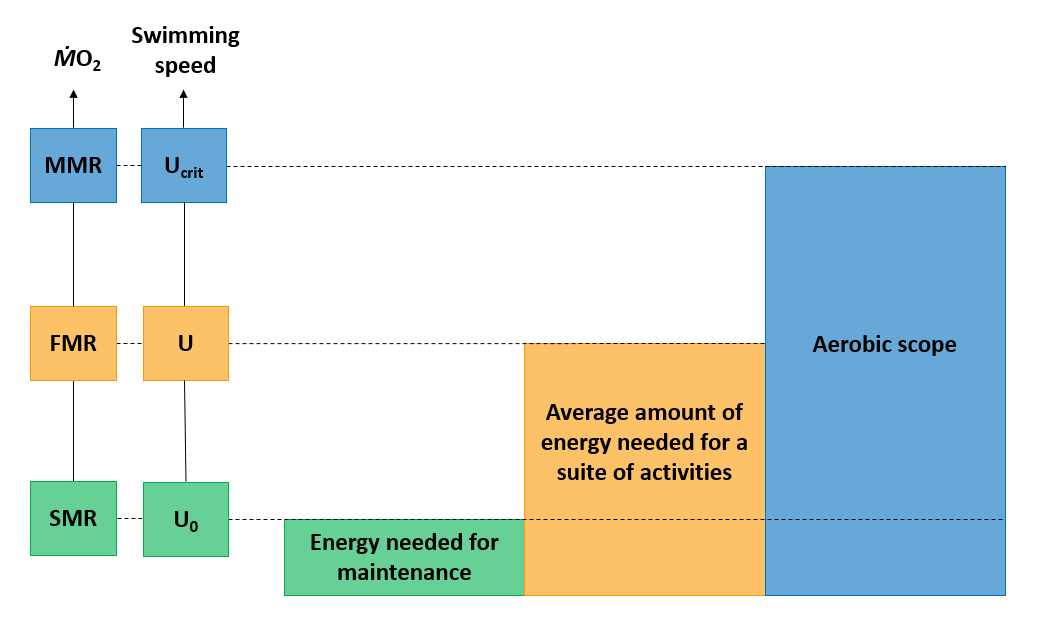
\includegraphics[width=14.99in]{../text/figures/figure1} \caption{testttt}\label{fig:unnamed-chunk-1}
\end{figure}

\hypertarget{methods}{%
\subsection{Methods}\label{methods}}

\hypertarget{model-species-and-study-system}{%
\subsubsection{Model species and study
system}\label{model-species-and-study-system}}

\noindent All data was collected in Mo'orea, French Polynesia, between
March 2018 and November 2018. We focused on seven fish species with
varying body size, trophic strategy, and behaviour: Cephalopholis argus
(Schneider, 1801), a large sedentary piscivore; Chaetodon ornatissimus
(Cuvier, 1831), an obligate coral feeder; Chromis iomelas (Jordan and
Seale, 1906), a small planktivore; Ctenochaetus striatus (Quoy and
Gaimard, 1825), a detrivore; Naso lituratus (Forster, 1801), a large
herbivore feeding on macroalgae; Odonus niger (Rüppell, 1836), a large
schooling planktivore; and Zebrasoma scopas (Cuvier, 1829), a herbivore
feeding on filamentous algae.

\hypertarget{standard-and-maximum-metabolic-rate-estimations-through-respirometry}{%
\subsubsection{Standard and maximum metabolic rate estimations through
respirometry}\label{standard-and-maximum-metabolic-rate-estimations-through-respirometry}}

\noindent To quantify SMR and MMR, we conducted intermittent-closed
respirometry experiments at 28°C (cf.~Steffensen, 1989; Clark et al.,
2013) on a total of 68 individuals of the seven study species, which
were collected in the lagoon (depth range XX-YYm) around Mo'orea with
hand nets and clove oil. After an acclimatisation and fasting period of
48 h in aquaria in the laboratory, the fish were transferred
individually to a water-filled tub at 28°C and manually chased by the
experimenter until exhausted (Norin and Malte, 2011; Clark et al.,
2012), after which they were placed in respirometry chambers submersed
in an ambient and temperature-controlled tank, where they were left for
\textasciitilde{}24 h. The intermittent respirometry cycles started
immediately after a fish was placed in its respirometry chamber and
consisted of a measurement (sealed) period followed by a flush period
during which the respirometry chambers were flushed with fully aerated
water from the ambient tank. Because fish were exhausted right before
entering the respirometry chambers, it is possible to measure the
approximate MMR. Depending on fish size, X to X respirometry chambers
ranging in volume (including tubes and pumps) from X to X L were run in
parallel, and measurement and flush periods lasted between X to X min
and X to X min, respectively. SMR was calculated as the average of the
10 \% lowest \(\dot{M}O_{2}\)values measured during the entire period,
after the removal of outliers (Chabot et al., 2016). MMR was calculated
from the slope of the first measurement period (see Supporting
Information Table 1) while SMR was calculated as the average of the 10\%
lowest \(\dot{M}O_{2}\)values measured during the entire
\textasciitilde{}24 h respirometry trial, after removal of any outliers
(Chabot et al., 2016).

\hypertarget{swimming-speed-estimations-through-stereo-video-analysis}{%
\subsubsection{Swimming speed estimations through stereo-video
analysis}\label{swimming-speed-estimations-through-stereo-video-analysis}}

\noindent We used two underwater stereo-video systems that were placed
on the seafloor during to record fish movements. Each video system had 2
cameras (GoPro Hero6 Black), spaced at 90 cm from each other at an angle
of approximately 6°. This method allows three-dimensional (3D)
measurements (Butail and Paley, 2012; Hughes and Kelly, 1996). To
analyse the recorded videos, we used VidSync, an open-source Mac
application providing accurate 3D measurements thanks to its
mathematical methods {[}described by Neuswanger et al. (2016){]}, which
allow the synchronisation, calibration, and navigation of videos. We
recorded calibration videos to correct for the nonlinear optical
distortion of the images due to camera lenses and underwater housings,
and to define the 3D coordinate system (x, y, z) used throughout the
analyses, to calculate the fishes' 3D positions. Errors in length
measurements through video analysis increase with distance from the
cameras (Neuswanger et al., 2016). Thus, for each underwater
stereo-video system, we fitted a linear regression model describing the
error in measurements in function of their distance from the nearest
camera, which we used to adjust all measurements of distances and fish
lengths (see Supporting Information Figure 1). We recorded twenty
stationary stereovideos between the 19th of November 2018 and the 12th
of December 2018. Videos were recorded at 12 to 14 m depth on the reef
slope at the Tiahura site in Mo'orea (17 ° 29 `00.6 " S, 149 ° 54' 20.9
" W) and at five different time-periods: 5:00--7:00, 8:00--10:00,
11:00--13:00, 14:00--16:00, and 17:00--18:00. Each recording lasted for
as long the battery lasted (\textasciitilde{}1 h). We then took
measurements during three 10 min sequences with intervals of 10 min
starting at the end of an acclimatisation period of 2 min to account for
the presence of divers, which could affect fish behaviour (Hill and
Wilkinson, 2004). We took measurements for all fishes visible by both
cameras for 3 to 5 s during the three 10 min sequences. For each
individual, fork length was measured three times from the videos as the
straight-line distance between the fish's head and its tail fork, and
three to five consecutive swimming speeds were measured as the distance
the fish moved over the 3 to 5 s. Final fish lengths and swimming speeds
were then calculated as the mean of the repeated measurements (see
Supporting Information Table 2). In total, we recorded lengths and
speeds for 634 fish.

\hypertarget{maximum-swimming-speed}{%
\subsubsection{Maximum swimming speed}\label{maximum-swimming-speed}}

\noindent We extracted maximum swimming speeds (Ucrit) from Fulton et
al. (2007). Ucrit was defined by Brett (1964) as the swimming speed at
which a fish becomes exhausted and stops swimming when it is exposed to
regular incremental changes in speed in an experimental flume. In these
experimental conditions, \(\dot{M}O_{2}\)measured at Ucrit corresponds
to the MMR (Norin and Clark, 2016). In Fulton et al. (2007), Ucrit of
192 individuals of five families and their corresponding lengths were
measured, and these measurements were then used in the present study
(see Supporting Information Table 3) to related maximum swimming speed
with body size at the family-level.

\hypertarget{data-analysis}{%
\subsubsection{Data analysis}\label{data-analysis}}

\noindent We quantified FMR and factorial scope for activity (FSA) by
combining multiple regression models, describing the relationships
between SMR and MMR with body mass, swimming speed (U), and maximum
swimming speed {[}Ucrit; from Fulton et al. (2007){]} with body size.
First, we used the respirometry data to fit a relationship between
either SMR or MMR and body mass using a Bayesian hierarchical model: ,

\noindent where is the species, is the type of metabolic rate (SMR or
MMR), is the global intercept of the regression; is the effect on the
intercept for each species and type of metabolic rate, is the global
slope of , is the effect on the slope of for each species. We obtained
the mean intercept and slope per species by summing global- and
species-level parameters. As MMR and SMR are dependent on each other
(Hayes and Garland, 1995), we assumed that their relationship with
organisms' weight is identical, but at different scales (i.e.~both have
the same metabolic scaling coefficient). Further, we used an informative
prior to define the global slope distribution: (West et. al, 1997). For
all other parameters, we used uninformative priors as defined by Bürkner
(2017). Second, using the data retrieved from the video analyses, we
fitted a hierarchical Bayesian regression model for estimating fish
swimming speed in function of body length: ,

\noindent where is the species, is the global intercept of the
regression, is the effect on the intercept for each species, is the
global slope of , is the effect on the slope of for each species. For
each species, their corresponding regression coefficients were estimated
by summing two effects of the model: the global parameter and the
species-specific effect on the global parameter. The student's
t-distribution was applied to build a robust regression, as the nature
of our data includes outliers (Motulsky and Brown, 2006). Thirdly, we
fitted a model, similar to the previous one to predict maximum swimming
speed in function of body length on a family level using data extracted
from Fulton et al. (2007): , , \noindent where is the family, is the
global intercept of the regression, is the effect on the intercept for
each family, is the global slope of , is the effect on the slope of for
each family. Here, we also applied the student's t-distribution and used
general uninformative priors.

\noindent Factorial aerobic scope, field metabolic rate and factorial
scope for activity calculations To estimate the fish's factorial aerobic
scope (FAS), we first estimated their and transforming their length (TL)
in weight (W) by using the following length-weight relationship (Froese
et al., 2014): where and vary per species (Froese and Pauly, 2019, see
Supporting Information Table 4). Then, we quantified individuals' and
using 1000 posterior samples of the parameters defined by model 1, based
on the corresponding weights. For each iteration, FAS was calculated as
(Fry, 1947; Killen et al., 2016). Finally we summarised the FAS per size
per species by taking means, standard deviations, and 95\% confidence
interval.

\noindent Factorial scope for activity (FSA) is the factor obtained by
dividing the fish's FMR (\(\dot{M}O_{2}\) at average speed U) by their
SMR. To describe the relationship between \(\dot{M}O_{2}\)and swimming
speed (U), Brett (1964) used the traditional exponential function: .
Here, we applied the logarithm-transformed form (Korsmeyer et al.,
2002): . Consequently, the following equation was used in this study to
determine individual FMR:

\noindent where we consider the slope . is the result of model 2
application for their corresponding length, as well as organisms' with
model 3 and their and with model 1. We did this for 1000 sample
iterations of the predicted swimming speeds.

\noindent Once FMR was determined, we calculated FSA with the following
equation: . We repeated this for each iteration and then summarised FSA
per species per size. We assumed that fish rested for 12 h, representing
the typical behavioural feature of sleep, common in many fish species
(Shapiro and Hepburn, 1976). As such, for all studied species we assumed
that they are active during the day and inactive during the night.

\hypertarget{scaling-up-to-assemblage-level}{%
\subsubsection{Scaling up to
assemblage-level}\label{scaling-up-to-assemblage-level}}

\noindent In 2016, reef fish communities were monitored in 13 sites on
the outer reef around Mo'orea using underwater visual census. During
each census a diver swam along a transect of 25m and counted all fishes
within a width of 2m. All fishes were identified to the species level
and their length was estimated to a preciscion of 1cm. Each transect
covered an area of 50 m², except Tiahura and Haapiti that covered an
area of 100 m² each. At each site, three transects were done, except for
Tiahura and Haapiti sites for which 4 and 2 transects were observed
respectively.\\
We extracted data for our model species from this database, which
resulted in 802 individuals across 7 species (Figure S2). Then, for each
site, we quantified the SMR and FMR for each individual using the
above-mentioned methodology. We then calculated the total SMR and FMR of
the fish assemblage per site, by adding up individual estimates.

\hypertarget{results}{%
\subsection{Results}\label{results}}

\hypertarget{standard-and-maximum-metabolic-rate-predictions}{%
\subsubsection{Standard and maximum metabolic rate
predictions}\label{standard-and-maximum-metabolic-rate-predictions}}

\noindent Our Bayesian model (model 1) was able to accurately predict
SMR and MMR in function of the body mass and the species identity. Model
1 is described by the following equation: . For the intercept, the 95 \%
confidence interval of the distribution lies between −5.6 and −4.65 g O2
d−1. The 95\% confidence interval of the slope distribution (i.e.~the
metabolic scaling coefficient) lies between 0.69 and 0.81. This model
has a Bayesian R² of 0.97 and its residual variance (ơ) is equal to
0.27. For each studied species, we obtained the fitted regression of a
fish's SMR and MMR by adding the species-specific effects (Figure 2, see
Supporting Information Table 5). The average slope values per species
varied between 0.74 and 0.76.

\begin{verbatim}
## Registered S3 method overwritten by 'xts':
##   method     from
##   as.zoo.xts zoo
\end{verbatim}

\begin{figure}
\centering
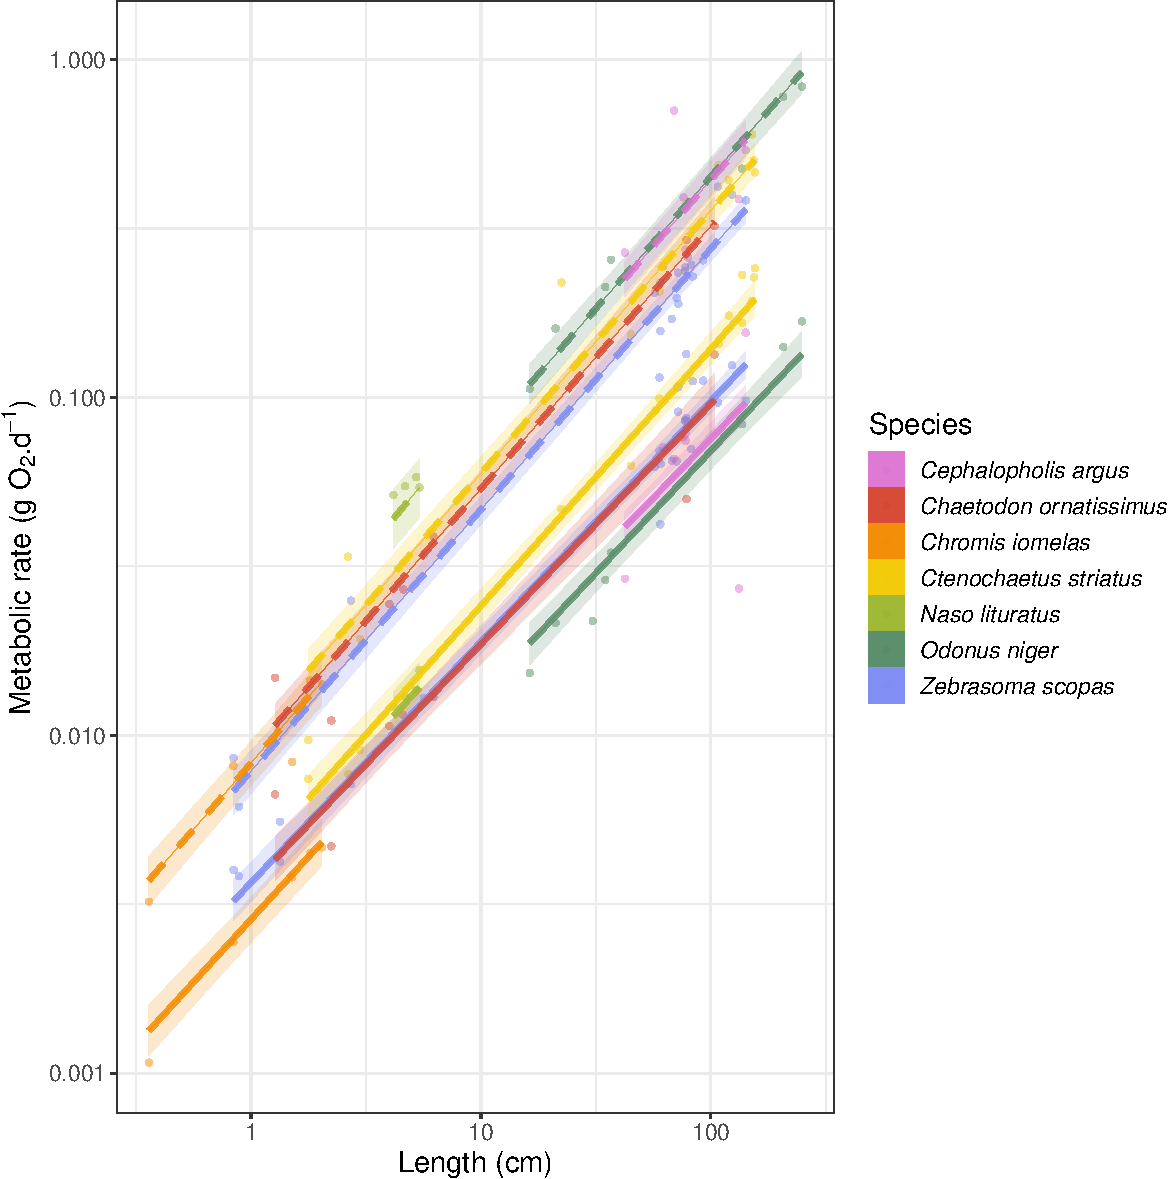
\includegraphics{main_text_files/figure-latex/unnamed-chunk-2-1.pdf}
\caption{testttt}
\end{figure}

Figure 2. Linear regressions between logarithm-transformed metabolic
rate (g O2 d−1) and weight (g) for the study species, predicted by model
1. Dots are empirical respirometry data. Solid and dotted lines
respectively represent MMR and SMR predicted mean values per species of
the response distribution for model 1. Grey areas are the confidence
intervals at 95\% of the regression lines.

\noindent The confidence interval at 95\% of SMR predictions on the
individual-level is estimated between 0.12 and 0.17 g O2 d−1, while the
95\% confidence interval of individuals' MMR predictions is defined
between 0.52 and 0.74 g O2 d−1 across all studied species and size
classes.

\hypertarget{swimming-speed-predictions}{%
\subsubsection{Swimming speed
predictions}\label{swimming-speed-predictions}}

\noindent  The Bayesian model to predict swimming speed in function of
body size and species identity (model 2) is described by the following
equation: . The 95 \% confidence interval of the intercept lies between
0.52 and 2.86 s−1, and the 95\% confidence interval for the slope lies
between 0.16 and 1.04. Model 2 has a bayesian R² of 0.57 and its
residual variance (ơ) is equal to 0.37. The average slope values per
species varies between 0.18 and 0.97 (Figure 3, see Supporting
Information Table 6).

\begin{figure}
\centering
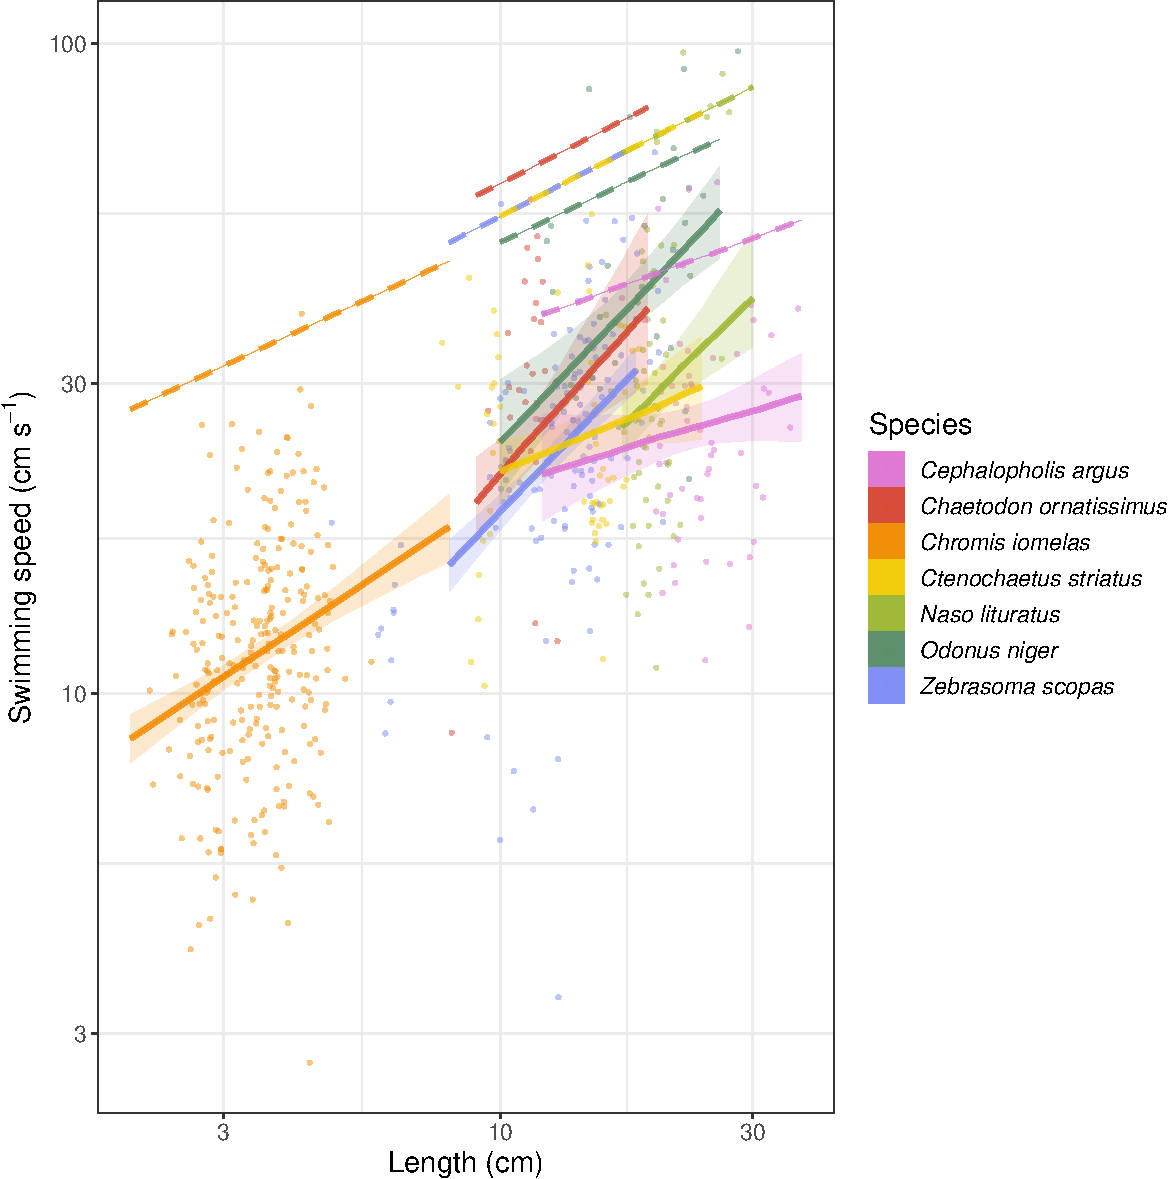
\includegraphics{main_text_files/figure-latex/unnamed-chunk-3-1.pdf}
\caption{testttt}
\end{figure}

Figure 3. Linear regressions between logarithm-transformed speed (cm
s−1) and length (cm) for the 7 studied fish species. Dots are length and
swimming speed of individuals measured through stereovideo analysis.
Solid lines and grey areas represent the mean values, and associated
95\% confidence interval, of swimming speeds predicted by a model for
each species .

At the individual scale, the 95\% confidence interval of swimming speed
predictions varies between 28.5 and 32.4 cm s−1 across all studied
species and all size classes.

\hypertarget{maximum-swimming-speed-predictions}{%
\subsubsection{Maximum swimming speed
predictions}\label{maximum-swimming-speed-predictions}}

\noindent Fulton et al. (2007) estimated maximum swimming speed of
several reef fish families with a flow chamber. Using those data, we
applied a Bayesian model (model 3) to estimate maximum swimming speed of
the fish from our study according to their body size and family
identity.

\noindent Model 3 has a bayesian R² of 0.35 and is described by the
following equation: . The confidence interval at 95\% of maximum
swimming speed predictions on the individual-level is estimated between
57.8 and 64.2 cm s−1 across all studied families and all size classes
(see Supporting Information Figure 2 and Table 7).

\hypertarget{field-metabolic-rate-factorial-aerobic-scope-and-factorial-activity-scope-estimations}{%
\subsubsection{Field metabolic rate, factorial aerobic scope and
factorial activity scope
estimations}\label{field-metabolic-rate-factorial-aerobic-scope-and-factorial-activity-scope-estimations}}

\noindent  For all studied species, we estimated FMR, FAS, and FSA at
all size classes corresponding to the sizes observed in the Mo'orea
monitoring dataset of year 2016. Across all study species and all size
classes, the 95\% confidence interval of FMR estimations varied between
0.19 and 0.27 g O2 d−1 at the individual scale, and the ones of FAS and
FSA varied between 4.04 and 4.73 g O2 d−1 and between 1.5 and 1.64 g O2
d−1, respectively. Figure 4 presents FAS and FSA mean values for the
median length per species.

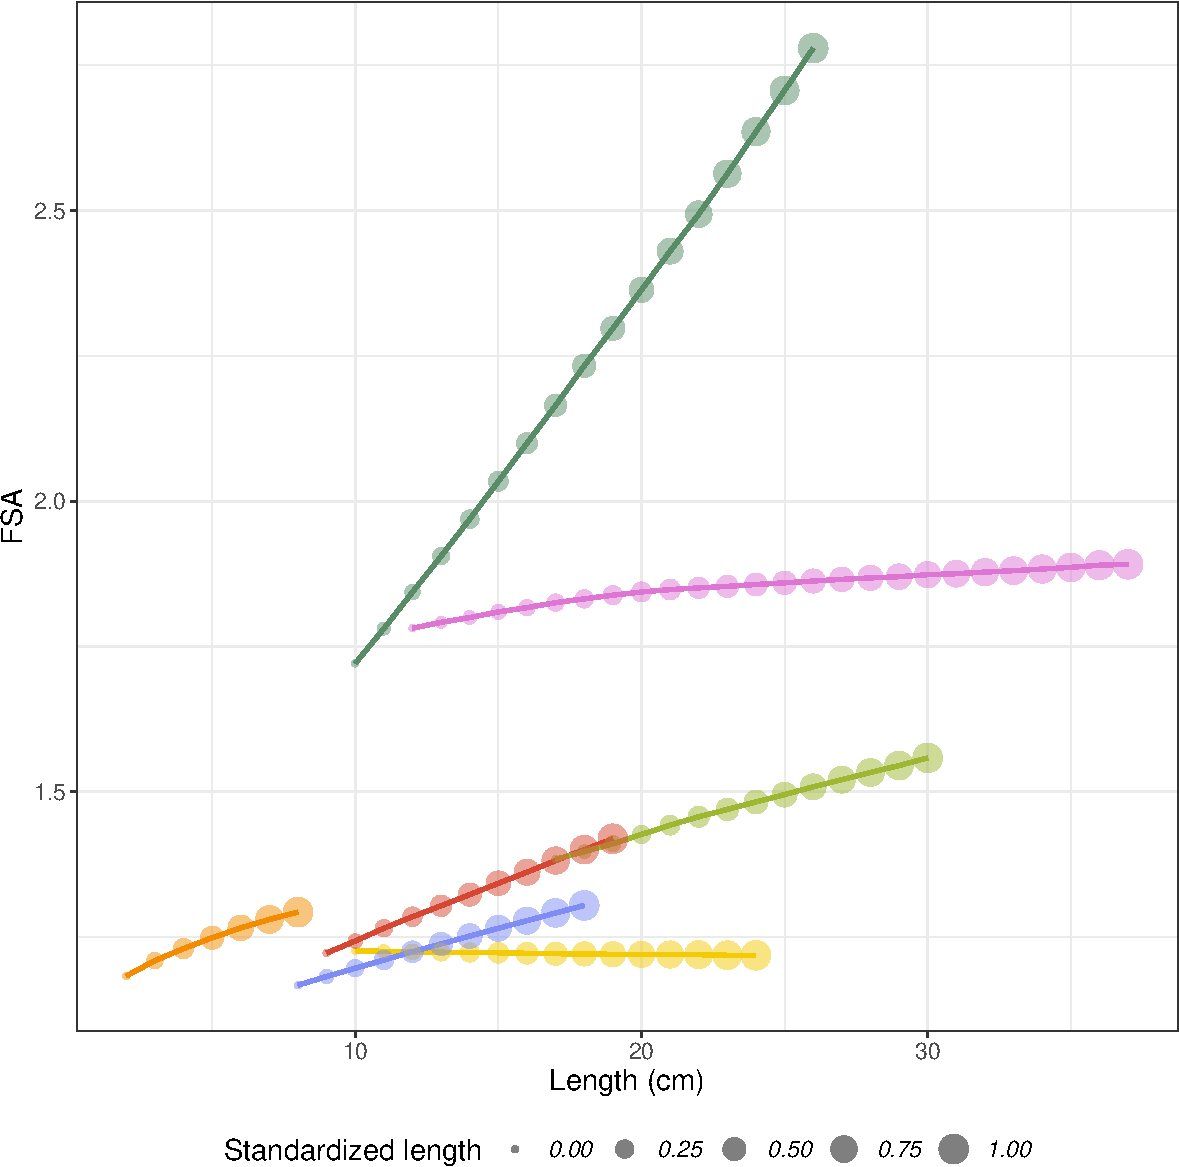
\includegraphics{main_text_files/figure-latex/unnamed-chunk-4-1.pdf}
Figure 4. Circles represent estimates of factorial aerobic scope and
factorial scope for activity for the median length (cm) per studied
species. Error bars represent lower and upper confidence intervals at
95\%.

\noindent  Standard metabolic rate and field metabolic rate scaling up
to the community-level The total SMR (± SD) of each fish community per
studied site are quantified between 0.026 ± 0.009 and 0.325 ± 0.021 g O2
m−2 d−1 across all sites (Figure 5). Further, the total FMR (± SD)
varies between 0.036 ± 0.014 g O2 m−2 d−1 and 0.465 ± 0.07 g O2 m−2 d−1.
The variation in total SMR and FMR at the community-level between sites
is related to the abundance of the studied fish assemblages per site
(see Supporting Information Figure 3).

\begin{figure}
\centering
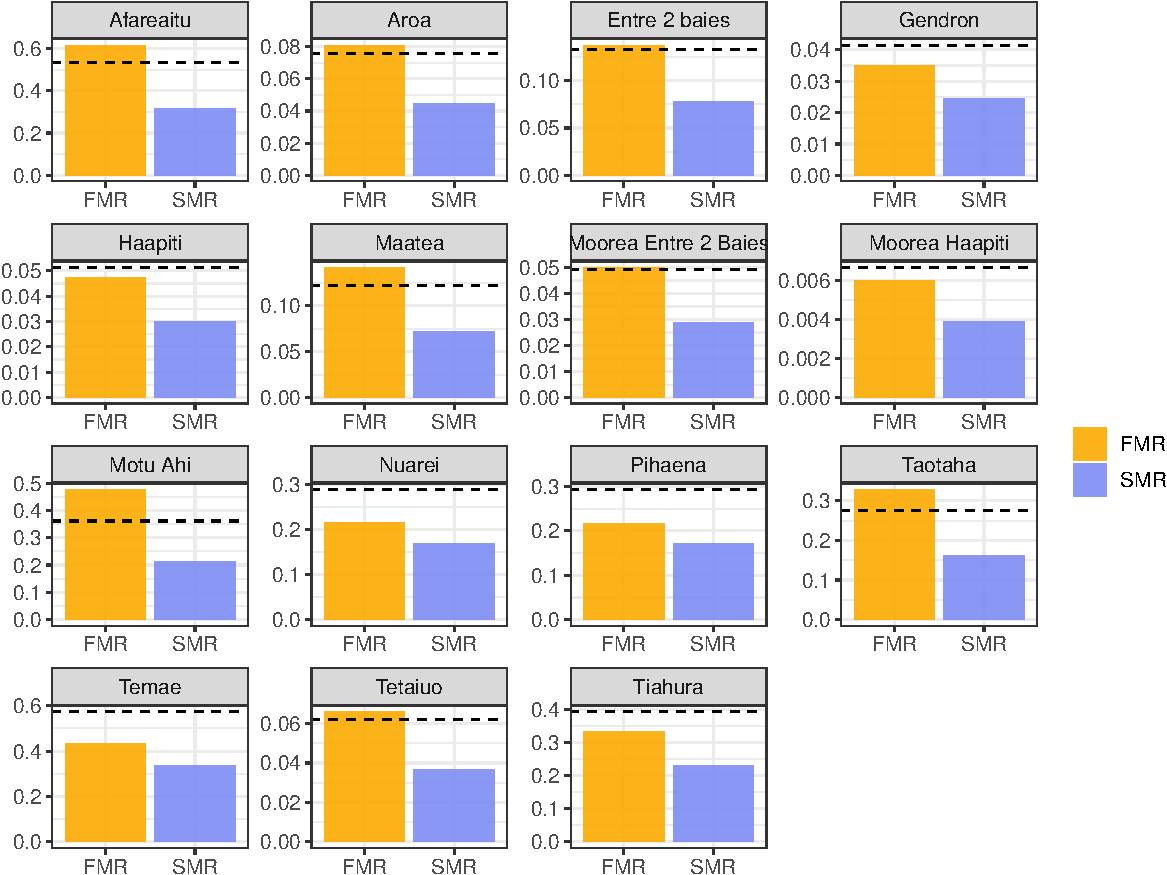
\includegraphics{main_text_files/figure-latex/unnamed-chunk-5-1.pdf}
\caption{teest}
\end{figure}

\noindent  Afareaitu, Maatea, Motu Ahi, Taotaha and Tetaiuo have a total
FMR about twice as high as the total SMR, and these are sites where C.
argus and O. niger constitutes dominate the reef fish assemblage. On the
contrary, sites dominated by C. striatus (50 to 95\% of the total reef
fish abundance) have a total FMR 1.27 to 1.41 times higher than the
total SMR (i.e.~Nuarei, Pihaena, Temae, Tiahura). Do we quantify the
metabolic scaling coefficient of FMR ifo biomass? Can be an extra thing
to add to the results/discussion..

\hypertarget{discussion}{%
\subsection{Discussion}\label{discussion}}

\noindent Field metabolic rate is an essential process that strongly
influences the flux of elements in fishes and communities, yet, it is
rarely considered at the community level due to the lack of quantitative
data on the activity of dominant fish species (Treberg et al., 2016).
Here, we tackle this issue by coupling experimental data on metabolic
rates with field observation through stereo-video analysis. To our
knowledge, this is the first time this method is used to quantify
activity rates of fishes. We exemplify our approach with a case study of
the physiology, swim speed performance, behavuoral activity, and
relative abudance of 7 common coral reef fish species. We show that the
activity scope of these study species varies between 1.25 and 2, and is
highly correlated with the aerobic scope. Moreover, we demonstrate how
ignoring activity rates underestimates the metabolic rate in assemblages
of reef fishes that exhibit varying levels of activity and relative
abundance on coral reefs. While our results are based only seven model
species, they commonly found on coral reefs across the Indo-Pacific, and
span a range of trophic levels from higher order carnivore to
planktivores, corallivores and herbivore/detritivore. We argue that
stereo-video analysis provides an opportunity to estimate field
metabolic rates of fishes in the wild, when combined with experimental
metabolic data.

\noindent Metabolic rates of our study species vary predictably with
body mass, in accordance with the MTE (Brown et al., 2004). The
dependence of metabolic rates on body size is demonstrated in many
studies and our results add to the existing literature (Schmidt-Nielsen,
1990; White and Seymour, 2003, 2004). The average slope value of our
model describing this relationship is equal to the allometric exponent
of 0.75 predicted by the model built by West et al. (1997) on the
allometric scaling law. Moreover, the range of our FAcS estimations
includes the estimates of Trudel and Boisclar (1996) that showed that
the average FMR of dace is 1.9 times SMR using both bioenergetic and
behaviour approaches. However, other studies quantified FMR up to three
to five-fold than SMR in some fish species, and up to nine-fold in tunas
(Brill and Bushnell, 1991; Chabot et al., 2016).

\noindent Both the swimming speed and the aerobic capacity of fishes
affect their field metabolic rate and thus their factorial activity
scope (Clark et al.~2013). In our case study, the two fishes with the
highest factorial activity scope are O. niger and C. argus, due to their
high aerobic scope. They use about one third of their aerobic capacity
in their natural environment. On the other hand, fishes with a low
factorial activity scope (i.e.~C. iomelas, C. ornatissimus, C. striatus,
and Z. scopas) are more active, relative to their maximum swimming
capacities. Therefore, their factorial activity scope is closer to their
factorial aerobic scope.

\noindent The interspecific variability of swimming speed, aerobic
capacity, and the field metabolic rate in fishes is influenced by
ecological traits, such as size, trophic level and habitat use. Small
fishes tend to be less performant than bigger ones (Brown et al.~2004).
Further, larger sizes in fishes provide physiological advantages, such
as swimming abilities permitting the exploitation of larger home ranges
(Nash et al., 2015). Furthermore, predators tend to have a higher
metabolic capacity, compared to herbivores, and pelagic fishes than
benthic fishes, as both have high locomotory demands because of their
mobility in a 3D environment (Killen et al., 2016; Nash et al., 2015).

\noindent When scaling up metabolic rates of fishes to the community, as
expected, the widely used SMR underestimates the actual metabolic rate
of communities. Our community-level analyses indicate that total
estimated metabolism of reef fish communities increase on average
two-fold compared to the total SMR to its corresponding total FMR. This
seems evident as SMR does not consider the spontaneous activity of
individuals (Chung et al., 2019; Clark et al., 2013). The variation
among sites in terms of the difference between the total SMR and FMR can
be explained by differences in community structure (Brown et al., 2004).
Communities, characterised by a high abundance of predators and/or
pelagic fishes present the largest differences between FMR and SMR
(e.g.~Afareaitu, Maatea, Motu Ahi, Taotaha, and Tetaiuo). Even though
our case study only includes a very low proportion of the actual fish
communities in Mo'orea, we show that species composition determines the
total field metabolic rate of communities. As a consequence, only
looking at SMR may fail to reveal differences in community-level
metabolic rates between sites. For example, Tetaiuo and Aroa have a very
similar SMR, but due the difference in species composition the FMR in
Aroa is considerably higher. Thus, the consideration of FMR of fishes is
not negligible when quantifying metabolic rates of fish communities.

\noindent Some limitations have to be considered. Firstly, we used
family-level maximum swimming speeds to reconstruct the relationship
between metabolic rate and swimming speed. This may introduce some bias
into the calculations, as different species were used in Fulton et al.
(2007). For all our studied species, maximum swimming speeds should
ideally be measured using the critical swimming speed protocol in
respirometry (Brett, 1964).\\
Further, we assumed that SMR is correlated with MMR by a physiological
linkage, FAeS being constant independently of body size (Hayes and
Garland, 1995). Many studies found no relationship between FAeS and body
size within species (Cutts et al., 2002; Wieser and Forstner, 1986), but
others reported FAeS variation according to the mass (Killen et al.,
2007). Divergent results across studies can be explained by the variety
of studied size ranges. Here, FAeS was estimated on adult reef fishes,
contrary to Killen et al. (2007) who measured SMR and MMR of fish
larvae. However, more work is needed to disentangle the relationship
between FAeS and body size. Finally, we quantified FAcS assuming that
fishes' spontaneous swimming varies at the daily scale with nocturnal
resting periods. However, there are day-active as well as night-active
species of fish (Zhdanova and Reebs, 2006). All our studied families are
diurnal families, except for Serranidae (Hobson, 1965). In fact,
groupers can be nocturnally active (Mourier et al., 2016). Thus, our
assumption can cause potential underestimations of FAcS in C. argus. Our
stereo-video recordings are unadapted to quantify fish swimming speeds
during the night, as measurements are inaccurate and imprecise with the
darkness and bad visibility (Neuswanger et al., 2016). Infrared lighting
in stereo-video recordings could be used to observe nocturnal behaviour
and movements in fishes (Bassett and Montgomery, 2011).

\noindent Despite these few limitations, our proposed method may help
fill the knowledge gap on field metabolic rates in fishes. Data is
scarce because it is challenging to observe the fishes in the field.
Laboratory techniques have been developed and used to quantify FMR,
however they are generally destructives or biased (Chung et al., 2019;
Treberg et al., 2016). The development of open-source software to
analyze videos demands a high sampling effort but provides the
possibility to quantitatively measure activity of fishes in their
environment. Thanks to the accuracy and the non-destructive nature of
stereo-video techniques, fish activity and behaviour are more and more
studied accurately in their natural environment (Bassett and Montgomery,
2011; Boisclair and Sirois, 1993; Guénard et al., 2008).

\noindent Anthropogenic stressors such as overfishing and climate change
are affecting fish communities at an unprecedented scale. In recent
times, the concern is growing that impoverished fish communities may not
be able to sustain ecosystem functioning and provide the ecosystem
services that are indispensable for human well-being. In order to take
the pulse of the functioning of a community, it is essential to quantify
key ecosystem processes such as nutrient cycling, herbivory, predation,
growth, etc (Brandl et al.~2019). The metabolic rate is an essential
component to estimate all of these processes. As the activity scope is
an important determinant of the field metabolic rate, we need more
research in order to study the role of fish in ecosystem functioning.

\hypertarget{references}{%
\subsection{References}\label{references}}



\end{document}
